

\chapter{Dati geometrici}
\begin{center}
\begin{tabular}{|c|c|c|c|c|c|c|c|}
\midrule
\textit{Solenoide} & $n$ & $R_{int}$ & $R_{ext}$ & $R_{medio}$ & $l_{circonferenza}$ & $h$ & $A_{sezione}$  \\
		   & 322 & 0,05	 & 0,0937  & 0,07185 & 0,451446864 & 0,0225 &	0,00098325 \\
 \midrule
\end{tabular}
\end{center}


\begin{center}
\begin{tabular}{|c|c|c|c|c|}
\midrule
\textit{Capacità} & $R_{int}$ (cm) & $R_{ext}$ (cm) & $lunghezza$ (cm) & $spessore piastre$ (cm)\\
   & 5.89 & 3.546  & 40  & 0.31 \\
%?? nel file ods ci sono altre misure per gli stessi campi!
 \midrule
\end{tabular}
\end{center}

\subsubsection{Misura della lunghezza d'onda del laser}

Misuriamo c dalla relazione:
\begin{equation}
 c=\frac{1}{sqrt{LC}}
\end{equation}
pertanto misuriamo la frequenza di risonanza di un cricuito RLC, per differenti configurazioni.


\begin{comment}
Costruiamo un circuito RLC. Nota: il condensatore risente molto delle fluttuazioni, per cui lo colleghiamo a terra, per ridurle il più possibile.

Frequenze di risonanza intorno ai 500 kH (nota: è un minimo -> potenziale ai capi di LC)
\end{comment}

\subparagraph*{Configurazione 1}
\begin{sagesilent}
#Fit per stimare i parametri -> Frequenza di risonanza: -b/2a

#Carico file
raw = np.recfromcsv('dati/EM/par38.csv')

#Seleziono dati per il fit
batch1 = raw[raw['freq']>675]
batch2 = batch1[batch1['freq']< 695]

#Carico negli array i dati giusti
freq = batch2['freq']
volt = batch2['vout']
yerr = batch2['errv']



def funz(x,a,b,c):
    return a*x^2+b*x+c

def func(P,x):
    return funz(x,P[0],P[1],P[2])

mymod = odr.Model(func)
mydata = odr.RealData(freq,volt)
myfit = odr.ODR(mydata,mymod,beta0=[1.,1.,1.],maxit=1000)
myout = myfit.run()

plt.clf()
xin = np.arange(min(freq),max(freq),1)
yin = func(myout.beta,xin)
plt.plot(freq,volt,'ro')
plt.errorbar(freq,volt,yerr,np.zeros_like(yerr),fmt=None)
plt.plot(xin,yin,'b--')
plt.grid(True)

#trovo minimo dai parametri x=-b/2*a
min1 = -myout.beta[1]/(2*myout.beta[0]) 

#stampo minimo su grafico
s = repr(round(min1,2))+" $(Hz)$"
plt.text(680,0.70,s,fontsize=12,bbox=dict(facecolor='red',alpha=0.1))

plt.savefig("grafici/prova.png",dpi=300)

\end{sagesilent}

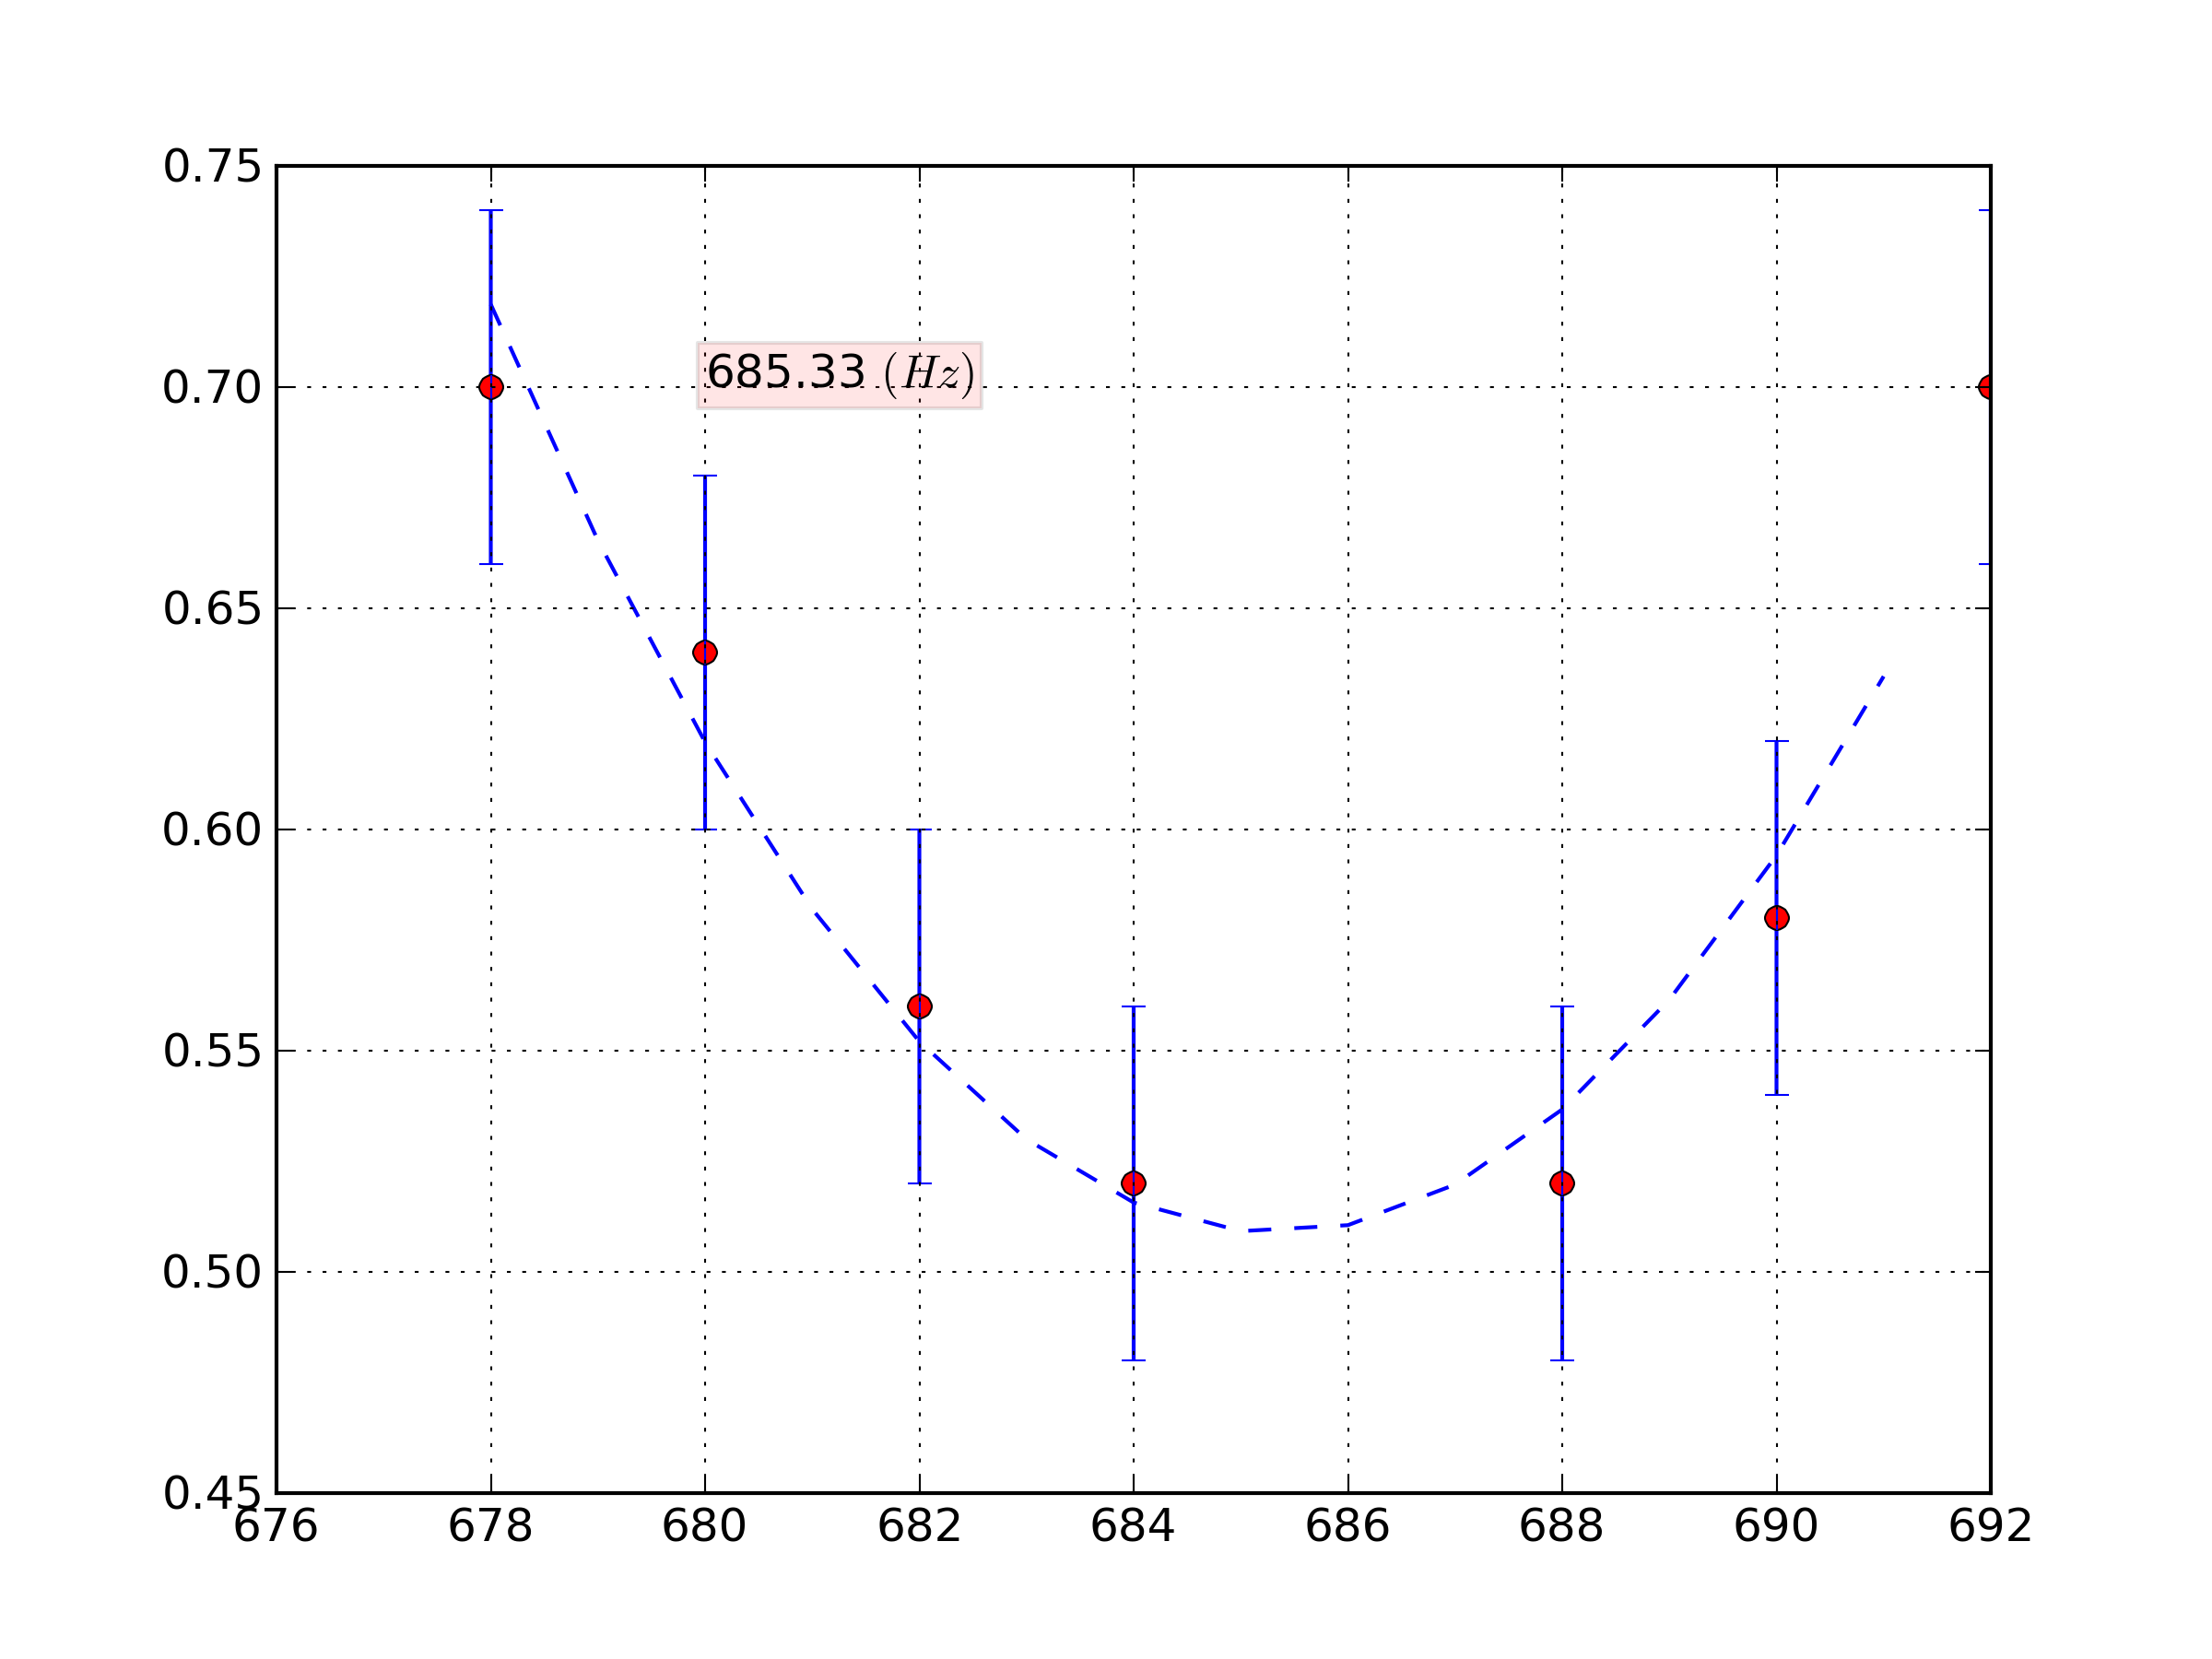
\includegraphics[scale=0.75]{grafici/prova.png}


\begin{comment}
\begin{center}
\sagestr{stampa_dati(dati, r'$\omega$ (rad) & $\V_{out}$ (nm) & $\sigma_{V_{out}}$ (nm)' )}
\end{center}
\end{comment}



\chapter{Analisi con capacità parassite in serie}
\chapter{Analisi con capacità parassite in parallelo}


